% Provenance (never printed): see sources/outline_sources.md (Year 3: the heat
% equation, half-space and plate cooling models, heat flow against age,
% continental geotherms, thermal subsidence). Brief: sources/book5/BRIEFS.md,
% ch. 5. Curves from figdata/bachelor-3/plate_cooling.py (models; Seton et al.
% 2020 age grid and ETOPO1, read only) and continental_geotherm.py.
% Exercise and problem values in the Book 5 scratch calculator calc/ch05.py.
\chapter{Model Termal Litosfer}\label{ch:b3:lithosphere-thermal-models}

Jika kamu berlayar menjauhi punggungan tengah samudra, dasar laut makin dalam: sekitar
\qty{2.5}{km} di sumbu punggungan, dan lebih dari \qty{5}{km} di bawah dasar
laut tertua. Tidak ada yang ditambahkan ke lempeng atau diambil darinya; ia hanya
mendingin, menyusut, dan tenggelam. Dasar laut adalah termometer bagi lempeng
di bawahnya, dan probe aliran panas yang ditancapkan ke sedimennya
membaca pendinginan yang sama dari atas. Bab ini menyelesaikan pendinginan lempeng dengan dua cara, sebagai
setengah-ruang dan sebagai lempeng berhingga tebal, lalu membandingkan keduanya dengan kedalaman
dasar laut sungguhan dan aliran panasnya, kemudian beralih ke benua,
yang panasnya sebagian berasal dari kerak mereka sendiri.
% ledger: ps77:depth-age

\begin{recall}
Persamaan difusi untuk panas, $\partial T/\partial t = \kappa\nabla^2T$,
dengan konduktivitas termal $k$ dan difusivitas termal $\kappa =
k/(\rho c)$, ada di buku fisika; deret Fourier dan fungsi galat
$\operatorname{erf}x = (2/\sqrt\pi)\int_0^xe^{-u^2}\,\mathrm du$ dibahas dalam
volume universitas buku matematika. Aliran panas, produksi panas
radiogenik, geoterm, skala waktu konduktif $L^2/\kappa$, lapisan
batas termal dan litosfer termal didefinisikan dalam volume Tahun 1,
dalam bab tentang anggaran panas Bumi; isostasi dalam bab tentang isostasi
dan anomali gravitasi; hukum kedalaman--umur $d = d_r + C\sqrt t$ dibuktikan dalam
bab tentang celah, punggungan, dan tepi pasif, dengan menerima profil suhu
yang diturunkan bab ini. Model peregangan cekungan, penurunan pascacelah
serta konstanta waktu termal ada di volume Tahun 2, dalam bab
tentang cekungan sedimen.
\end{recall}

\section{Konduksi, adveksi, dan rasionya}

Panas dalam litosfer bergerak dengan dua cara: ia berdifusi menuruni
gradien suhu, dan ia terbawa oleh batuan yang bergerak, misalnya lempeng yang meninggalkan punggungan, gunung
yang tererosi sedang terangkat, magma yang naik. Mana yang menang bergantung pada satu
bilangan saja.

\begin{definition}[Bilangan Péclet termal]\label{def:b3:lithosphere-thermal-models:peclet}
Untuk batuan yang bergerak dengan kecepatan $u$ melintasi panjang $L$, \emph{bilangan Péclet
termal}\index{bilangan Péclet termal} adalah
\[
  \mathrm{Pe} = \frac{uL}{\kappa},
\]
rasio waktu konduktif $L^2/\kappa$ terhadap waktu adveksi $L/u$.
Adveksi mendominasi ketika $\mathrm{Pe} \gg 1$, konduksi ketika
$\mathrm{Pe} \ll 1$.
\end{definition}

Lempeng yang meninggalkan punggungan dengan kecepatan \qty{25}{mm/yr} memiliki, pada jarak
\qty{95}{km}, $\mathrm{Pe} \approx 94$ dengan $\kappa = \qty{0.8e-6}{m^2.s^{-1}}$:
panas terbawa ke samping oleh lempeng jauh lebih cepat daripada berdifusi ke samping.
Karena itu, setiap kolom vertikal lempeng mendingin seakan sendirian, melalui
konduksi vertikal ke dasar laut yang dingin, dengan umur $t$ menyatakan waktu sejak
ia meninggalkan sumbu. Hal itu mengubah masalah dua dimensi menjadi satu dalam
kedalaman dan waktu.

\section{Setengah-ruang yang mendingin}

\begin{definition}[Model pendinginan setengah-ruang]\label{def:b3:lithosphere-thermal-models:half-space}
Yang disebut \emph{model pendinginan setengah-ruang}\index{model pendinginan setengah-ruang} dari
litosfer samudra memperlakukan setiap kolom sebagai setengah-ruang $z \ge 0$ dengan
difusivitas seragam, pada suhu seragam $T_m$ mantel ketika ia meninggalkan
sumbu punggungan; permukaannya dijaga sejak saat itu pada suhu $T_0$ dasar
laut, tanpa produksi panas dan tanpa dasar.
\end{definition}

\begin{theorem}[Geoterm fungsi galat]\label{thm:b3:lithosphere-thermal-models:erf}
Dalam \omterm{def:b3:lithosphere-thermal-models:half-space}{model pendinginan setengah-ruang}, suhu pada kedalaman $z$ di bawah
dasar laut berumur $t$ adalah
\[
  T(z, t) = T_0 + (T_m - T_0)\operatorname{erf}\frac{z}{2\sqrt{\kappa t}} .
\]
Inilah \emph{geoterm fungsi galat}\index{geoterm fungsi galat}.
\end{theorem}

\begin{proof}
Misalkan $\theta = (T - T_0)/(T_m - T_0)$; ia memenuhi $\partial\theta/\partial t =
\kappa\,\partial^2\theta/\partial z^2$ dengan $\theta(z, 0) = 1$ untuk $z > 0$ dan
$\theta(0, t) = 0$ untuk $t > 0$. Soal ini tidak memiliki skala panjang sendiri:
jika $\theta(z, t)$ adalah solusi, begitu pula $\theta(\lambda z, \lambda^2t)$ untuk setiap
$\lambda > 0$, dengan nilai awal dan batas yang sama; karena solusinya
tunggal, $\theta$ bergantung pada $z$ dan $t$ hanya melalui $\eta = z/(2\sqrt{\kappa
t})$. Jika ditulis $\theta = f(\eta)$, dengan $\partial\eta/\partial t = -\eta/(2t)$ dan
$\partial\eta/\partial z = 1/(2\sqrt{\kappa t})$,
\[
  -\frac{\eta}{2t}f'(\eta) = \kappa\,\frac{f''(\eta)}{4\kappa t},
  \qquad\text{maka}\qquad f'' + 2\eta f' = 0 .
\]
Oleh karena itu $f' = Ae^{-\eta^2}$ dan $f = A\int_0^\eta e^{-u^2}\,\mathrm du + B$. Syarat
permukaan, pada $\eta = 0$, memberikan $B = 0$; syarat awal, yang
berlaku di setiap kedalaman saat $t \to 0$, yakni saat $\eta \to \infty$, memberikan
$A\sqrt\pi/2 = 1$. Jadi $f = \operatorname{erf}\eta$.
\end{proof}

Suhu pada kedalaman tertentu hanya bergantung pada $z/\sqrt t$: isoterm turun
sebanding dengan akar umur, dan lapisan dingin pada \qty{40}{Ma} dua kali
lebih tebal daripada pada \qty{10}{Ma}. Aliran panas permukaan diperoleh dengan diferensiasi.

\begin{proposition}[Hubungan aliran panas--umur]\label{prop:b3:lithosphere-thermal-models:heat-flow}
Dalam \omterm{def:b3:lithosphere-thermal-models:half-space}{model pendinginan setengah-ruang}, aliran panas melalui dasar laut berumur $t$
adalah
\[
  q(t) = k\,\frac{\partial T}{\partial z}\Big|_{z=0}
  = \frac{k(T_m - T_0)}{\sqrt{\pi\kappa t}} = \frac{C_q}{\sqrt t} .
\]
\end{proposition}

\begin{proof}
$\partial\operatorname{erf}(z/2\sqrt{\kappa t})/\partial z = (2/\sqrt\pi)
e^{-z^2/4\kappa t}/(2\sqrt{\kappa t})$, yang pada $z = 0$ bernilai $1/\sqrt{\pi\kappa
t}$.
\end{proof}

Dengan nilai-nilai model lempeng di bawah ($k = \qty{3.1}{W.m^{-1}.K^{-1}}$,
$T_m - T_0 = \qty{1450}{K}$, $\kappa = \qty{0.8e-6}{m^2.s^{-1}}$), $C_q =
\qty{505}{mW.m^{-2}.Ma^{1/2}}$, mendekati nilai 430 sampai
\qty{510}{mW.m^{-2}.Ma^{1/2}} yang dicocokkan dengan pengukuran global oleh berbagai
studi; kompilasi terbaru lebih memilih \num{490}. Aliran panas yang terukur pada
kerak samudra muda, namun, jauh meremehkan panas yang keluar darinya:
air laut yang beredar melalui kerak yang retak membawa sebagian panas keluar
lewat mata air panas, di luar jangkauan alat ukur. Pada kerak tua, pengukuran
mengikuti $1/\sqrt t$, dan taksiran kehilangan panas Bumi menggantikan
pengukuran pada kerak yang lebih muda dari \qty{66.5}{Ma} dengan $C_q/\sqrt t$.
% ledger: honda04:gdh1, b2dd10:half-space, dd10b5:hydrothermal

Volume Tahun 1 mengintegralkan profil yang sama terhadap kedalaman, melalui isostasi, untuk
memperoleh hukum kedalaman--umur, $d = d_r + C\sqrt t$ dengan $C = 2\rho_m\alpha(T_m -
T_0)\sqrt\kappa/\bigl(\sqrt\pi(\rho_m - \rho_w)\bigr)$ (gambar di bawah). Dengan
$\rho_m = \qty{3300}{kg.m^{-3}}$, $\rho_w = \qty{1030}{kg.m^{-3}}$ dan $\alpha =
\qty{3.1e-5}{K^{-1}}$, $C = \qty{370}{m.Ma^{-1/2}}$, dibandingkan dengan
\qty{350}{m.Ma^{-1/2}} yang dicocokkan pada dasar Samudra Pasifik Utara dan
Samudra Atlantik Utara yang lebih muda dari \qty{70}{Ma}.
% ledger: ps77:depth-age

\begin{omfigure}
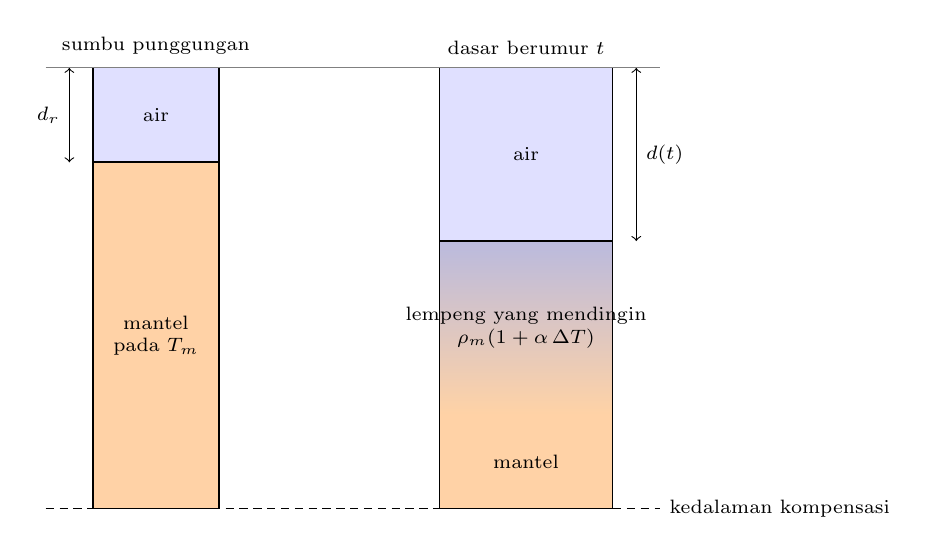
\begin{tikzpicture}[font=\small, x=1cm, y=1cm]
% schematic: two columns of equal mass above the compensation depth
\fill[blue!12] (0,0) rectangle (1.6,-1.2);
\fill[orange!35] (0,-1.2) rectangle (1.6,-5.6);
\fill[blue!12] (4.4,0) rectangle (6.6,-2.2);
\shade[top color=blue!35!gray!40, bottom color=orange!35] (4.4,-2.2) rectangle (6.6,-4.4);
\fill[orange!35] (4.4,-4.4) rectangle (6.6,-5.6);
\draw (0,0) rectangle (1.6,-5.6) (4.4,0) rectangle (6.6,-5.6);
\draw[densely dashed] (-0.6,-5.6) -- (7.2,-5.6) node[right, font=\scriptsize] {kedalaman kompensasi};
\draw[thick] (0,-1.2) -- (1.6,-1.2) (4.4,-2.2) -- (6.6,-2.2);
\node[font=\scriptsize] at (0.8,-0.6) {air};
\node[font=\scriptsize, align=center] at (0.8,-3.4) {mantel\\pada $T_m$};
\node[font=\scriptsize] at (5.5,-1.1) {air};
\node[font=\scriptsize, align=center] at (5.5,-3.3) {lempeng yang mendingin\\$\rho_m(1 + \alpha\,\Delta T)$};
\node[font=\scriptsize, align=center] at (5.5,-5.0) {mantel};
\draw[<->] (-0.3,0) -- (-0.3,-1.2) node[midway, left, font=\scriptsize] {$d_r$};
\draw[<->] (6.9,0) -- (6.9,-2.2) node[midway, right, font=\scriptsize] {$d(t)$};
\node[above, font=\scriptsize] at (0.8,0.05) {sumbu punggungan};
\node[above, font=\scriptsize] at (5.5,0.05) {dasar berumur $t$};
\draw[gray] (-0.6,0) -- (7.2,0);
\end{tikzpicture}

\par\smallskip{\small Isostasi lempeng yang mendingin: kolom di punggungan
dan kolom berumur $t$ memiliki massa yang sama di atas kedalaman kompensasi. Lempeng
yang mendingin dan lebih rapat tenggelam, dan air mengisi ruang di
atasnya.}\label{fig:b3:lithosphere-thermal-models:columns}
\end{omfigure}

\section{Model lempeng}

Dasar samudra tua berhenti menurun: di Samudra Pasifik Utara dan Samudra Atlantik
Utara, kedalaman menyimpang dari $\sqrt t$ antara 60 dan \qty{80}{Ma}, dan aliran
panas mendatar. Setengah-ruang terus mendingin tanpa henti; sesuatu harus menjaga
dasar lempeng tetap hangat.
% ledger: parsons:plate-model

\begin{definition}[Model pendinginan lempeng]\label{def:b3:lithosphere-thermal-models:plate}
Yang disebut \emph{model pendinginan lempeng}\index{model pendinginan lempeng} untuk
litosfer samudra menganggap setiap kolom sebagai lapisan $0 \le z \le L$ dengan
difusivitas seragam, pada suhu seragam $T_m$ saat meninggalkan punggungan, yang
permukaannya ditahan pada $T_0$ dan dasarnya ditahan pada $T_m$ sejak saat itu.
\end{definition}

\begin{theorem}[Deret suhu model lempeng]\label{thm:b3:lithosphere-thermal-models:plate-series}
Dalam \omterm{def:b3:lithosphere-thermal-models:plate}{model pendinginan lempeng}, dengan $T_0 = 0$,
\[
  T(z, t) = T_m\Bigl[\frac zL + \frac2\pi\sum_{n=1}^\infty\frac1n
  \sin\frac{n\pi z}{L}\,e^{-n^2t/\tau}\Bigr],\qquad
  \tau = \frac{L^2}{\pi^2\kappa} .
\]
Ini disebut \emph{deret suhu model lempeng}\index{deret suhu model lempeng}.
\end{theorem}

\begin{proof}
Keadaan tunak, yang tercapai saat $t \to \infty$, adalah profil linear $T_mz/L$.
Simpangan $u = T - T_mz/L$ memenuhi persamaan difusi dengan $u = 0$ pada
$z = 0$ dan $z = L$, dan mulai dari $u(z, 0) = T_m(1 - z/L)$. Dengan memisahkan
variabel, $u = Z(z)\Theta(t)$ memberikan $Z''/Z = \Theta'/(\kappa\Theta) = -\mu^2$;
syarat batas menyisakan $Z = \sin(n\pi z/L)$, $\mu = n\pi/L$, dan
$\Theta = e^{-n^2\pi^2\kappa t/L^2} = e^{-n^2t/\tau}$. Nilai awal menentukan
koefisien $b_n$ dari deret sinus $T_m(1 - z/L)$ pada $[0, L]$:
\[
  b_n = \frac2L\int_0^LT_m\Bigl(1 - \frac zL\Bigr)\sin\frac{n\pi z}{L}\,\mathrm dz
  = \frac{2T_m}{n\pi},
\]
dengan integrasi parsial. Menjumlahkan semua moda menghasilkan deret tersebut.
\end{proof}

Setiap moda meluruh dengan waktunya sendiri, $\tau/n^2$: harmonik yang lebih tinggi, struktur halus dari
langkah awal, lenyap lebih dulu, dan setelah waktu berorde $\tau$
hanya moda pertama yang tersisa. Pemisahan variabel yang sama memberikan aliran panas
dan, melalui keseimbangan isostatik pada gambar di atas, kedalamannya.

\begin{proposition}[Kedalaman dan aliran panas model lempeng]\label{prop:b3:lithosphere-thermal-models:plate-depth}
Dalam \omterm{def:b3:lithosphere-thermal-models:plate}{model pendinginan lempeng}, dengan massa jenis dan pemuaian pada hukum
kedalaman--umur,
\[
  q(t) = \frac{kT_m}{L}\Bigl[1 + 2\sum_{n=1}^\infty e^{-n^2t/\tau}\Bigr],\qquad
  d(t) = d_r + \frac{\rho_m\alpha T_mL}{2(\rho_m - \rho_w)}
  \Bigl[1 - \frac{8}{\pi^2}\sum_{n\ \text{ganjil}}\frac{e^{-n^2t/\tau}}{n^2}\Bigr].
\]
Saat $t \to \infty$, kedalaman menuju $d_r + \rho_m\alpha T_mL/\bigl(2(\rho_m -
\rho_w)\bigr)$ dan aliran panas menuju $kT_m/L$, keduanya secara eksponensial, dengan waktu
konstanta $\tau$.
\end{proposition}

\begin{proof}
Dengan menurunkan deret di $z = 0$, $\partial T/\partial z = (T_m/L)[1 +
2\sum e^{-n^2t/\tau}]$. Untuk kedalaman, keseimbangan isostatik memberikan $(\rho_m -
\rho_w)(d - d_r) = \rho_m\alpha\int_0^L(T_m - T)\,\mathrm dz$. Bagian linear
menyumbang $T_mL/2$; setiap moda menyumbang $-(2T_m/n\pi)e^{-n^2t/\tau}
\int_0^L\sin(n\pi z/L)\,\mathrm dz = -(2T_m/n\pi)(L/n\pi)(1 - \cos n\pi)
e^{-n^2t/\tau}$, yang nol untuk $n$ genap dan $-(4T_mL/n^2\pi^2)
e^{-n^2t/\tau}$ untuk $n$ ganjil. Dengan memfaktorkan $T_mL/2$ diperoleh kurung siku. Pada $t = 0$
suku itu lenyap, karena $\sum_{n\ \text{ganjil}}1/n^2 = \pi^2/8$.
\end{proof}

Model lempeng yang paling sesuai dengan kedalaman dan aliran panas global memiliki lempeng
\qty{95}{km} tebalnya, dengan dasar pada \qty{1450}{\celsius}, $\alpha =
\qty{3.1e-5}{K^{-1}}$ dan $k = \qty{3.1}{W.m^{-1}.K^{-1}}$, lebih tipis dan lebih panas
daripada sebelumnya \qty{125}{km} dan \qty{1350}{\celsius}. Dengan $\kappa =
\qty{0.8e-6}{m^2.s^{-1}}$, $\tau = \qty{36.2}{Ma}$; kedalaman mendatar pada
$2500 + 3104 = \qty{5604}{m}$ dan aliran panas pada \qty{47}{mW.m^{-2}}. Dasar
samudra muda tidak dapat membedakan kedua model: keduanya berbeda kurang dari satu meter pada
\qty{2}{Ma}, dan selisih \qty{100}{m} pada \qty{44}{Ma}. Seismologi memberikan
jawaban serupa: \omterm{def:b3:seismology-imaging:surface-waves}{gelombang Rayleigh} Pasifik paling sesuai dengan lempeng pendingin yang
ketebalan asimtotiknya 85 sampai \qty{95}{km}.
% ledger: honda04:gdh1, ps77:depth-age, fischer:lithosphere

\begin{omfigure}
\begin{tikzpicture}
\begin{groupplot}[group style={group size=1 by 2, vertical sep=2.3cm},
  omrecord, width=0.86\linewidth, height=0.42\linewidth, xmin=0, xmax=160,
  xlabel={umur dasar laut (Ma)}]
\nextgroupplot[omdepth, ylabel={kedalaman (km)}, ymin=0, ymax=130,
  title={(a) isoterm, tiap \qty{200}{\celsius}}, title style={font=\small},
  legend style={font=\scriptsize, at={(0.01,0.03)}, anchor=south west}]
% computed in figdata/bachelor-3/plate_cooling.py; ledger: honda04:gdh1
\addplot[omDef, thick] table[x=t, y=hs200] {figdata/out/bachelor-3-plate_cooling-isotherms.dat};
\addlegendentry{setengah-ruang}
\addplot[red!70!black, thick, densely dashed] table[x=t, y=pl200] {figdata/out/bachelor-3-plate_cooling-isotherms.dat};
\addlegendentry{lempeng, $L = \qty{95}{km}$}
\foreach \lev in {400,600,800,1000,1200,1400} {
  \addplot[omDef, thick, forget plot] table[x=t, y=hs\lev] {figdata/out/bachelor-3-plate_cooling-isotherms.dat};
  \addplot[red!70!black, thick, densely dashed, forget plot] table[x=t, y=pl\lev] {figdata/out/bachelor-3-plate_cooling-isotherms.dat};
}
\draw[gray] (axis cs:0,95) -- (axis cs:160,95);
\node[font=\scriptsize, anchor=north] at (axis cs:68,96) {dasar lempeng};
\node[font=\scriptsize, fill=white, inner sep=1pt] at (axis cs:150,14) {200};
\node[font=\scriptsize, fill=white, inner sep=1pt] at (axis cs:28,38.2) {1000};
\node[font=\scriptsize, fill=white, inner sep=1pt] at (axis cs:22,70.4) {1400};
\nextgroupplot[ylabel={aliran panas (\unit{mW.m^{-2}})}, ymin=0, ymax=300,
  title={(b) aliran panas}, title style={font=\small},
  legend style={font=\scriptsize, at={(0.98,0.97)}, anchor=north east}]
\addplot[omDef, thick] table[x=t, y=hs] {figdata/out/bachelor-3-plate_cooling-heat.dat};
\addlegendentry{setengah-ruang}
\addplot[red!70!black, thick, densely dashed] table[x=t, y=pl] {figdata/out/bachelor-3-plate_cooling-heat.dat};
\addlegendentry{lempeng}
\end{groupplot}
\end{tikzpicture}

\par\smallskip{\small Kedua model pendinginan dengan parameter pada teks.
(a) Kedalaman isoterm dari \qty{200}{\celsius} (atas) hingga
\qty{1400}{\celsius} (bawah): isoterm model setengah-ruang terus turun sebanding
dengan $\sqrt t$, isoterm model lempeng berhenti ketika profilnya menjadi linear. (b) Aliran
panas permukaan: model lempeng mendatar pada \qty{47}{mW.m^{-2}}, setengah-ruang
turun sebagai $1/\sqrt t$.}\label{fig:b3:lithosphere-thermal-models:isotherms}
\end{omfigure}

Dasar samudra yang sebenarnya dapat diletakkan pada grafik yang sama (gambar di bawah). Setiap sel
satu derajat lintang dan bujur yang umurnya diketahui diletakkan pada umur dan
kedalamannya; median setiap selang lima juta tahun naik seiring umur, sebagaimana model
menyatakan untuk \qty{40}{Ma} pertama, tetapi dasar yang teramati lebih dangkal daripada kedua
model, dan semakin dangkal seiring umur. Belum ada koreksi yang dilakukan: dasar tua
memiliki selimut sedimen yang lebih tebal, lebih dari satu kilometer, di bagian
Samudra Atlantik Utara yang lebih tua, yang membebaninya dan menaikkan puncaknya, dan dasar tua sempat
mengumpulkan gunung laut, dataran tinggi vulkanik, dan tonjolan titik panas. Penyesuaian yang
dipublikasikan lebih dulu menghilangkan beban sedimen dan tonjolan yang jelas. Hukum
kedalaman--umur dari volume Tahun 1 serta model lempeng di atas berasal dari
kedalaman yang telah dikoreksi tersebut.
% ledger: data:b5-depth-age, ps77:depth-age

\begin{omfigure}
\begin{tikzpicture}
\begin{axis}[omrecord, omdepth, width=0.86\linewidth, height=0.5\linewidth,
  xmin=0, xmax=180, ymin=2, ymax=6.5, xlabel={umur dasar laut (Ma)},
  ylabel={kedalaman (km)},
  legend style={font=\scriptsize, at={(0.5,-0.24)}, anchor=north, cells={anchor=west}},
  legend columns=2]
% computed in figdata/bachelor-3/plate_cooling.py; ledger: data:b5-depth-age, honda04:gdh1
\addplot[only marks, mark=*, mark size=1.3pt, black,
  error bars/.cd, y dir=both, y explicit]
  table[x=t, y expr=\thisrow{med}/1000, y error plus expr=(\thisrow{q3}-\thisrow{med})/1000,
  y error minus expr=(\thisrow{med}-\thisrow{q1})/1000] {figdata/out/bachelor-3-plate_cooling-bins.dat};
 \addlegendentry{teramati, median dan kuartil}
\addplot[omDef, thick] table[x=t, y expr=\thisrow{hs}/1000] {figdata/out/bachelor-3-plate_cooling-depth.dat};
\addlegendentry{setengah-ruang}
\addplot[red!70!black, thick, densely dashed] table[x=t, y expr=\thisrow{pl}/1000] {figdata/out/bachelor-3-plate_cooling-depth.dat};
\addlegendentry{lempeng, $L = \qty{95}{km}$}
\end{axis}
\end{tikzpicture}

\par\smallskip{\small Kedalaman dasar samudra terhadap umurnya: median dan
kuartil kedalaman sel satu derajat pada setiap selang lima juta tahun
(dasar laut lebih dalam dari \qty{1000}{m}, umur dari grid umur global, kedalaman
dari model relief global, tanpa koreksi untuk sedimen, gunung laut, atau tonjolan),
dengan kedua model pendinginan pada teks.}\label{fig:b3:lithosphere-thermal-models:depth-age}
\end{omfigure}

\begin{definition}[Penurunan termal]\label{def:b3:lithosphere-thermal-models:thermal-subsidence}
Yang disebut \emph{penurunan termal}\index{penurunan termal} adalah turunnya
permukaan litosfer seiring ia mendingin dan menyusut menuju
kesetimbangan termal, dengan ruang di atasnya terisi air atau sedimen; isostasi
mengubah panas yang hilang dari suatu kolom menjadi penurunannya.
\end{definition}

Dasar samudra adalah kasus murninya. Cekungan benua yang teregang adalah contoh
lainnya: litosfer yang menipis dengan faktor $\beta$ membawa astenosfer panas naik, dan
penurunan pascacelah pada volume Tahun 2 adalah pendinginan lempeng yang sama, dimulai
dari profil yang berbeda, dengan mode dan waktu peluruhan $\tau/n^2$ yang sama.
Karena itu, hanya mempertahankan mode pertama adalah pendekatan yang baik setelah mode-mode
yang lebih tinggi mereda, dan pendekatan yang buruk sebelumnya. Untuk dasar samudra pada model lempeng
di atas, suku pertama saja memberikan kedalaman dengan selisih dua meter setelah
\qty{20}{Ma}, tetapi terlalu dalam \qty{84}{m} pada \qty{5}{Ma}.

\section{Geoterm benua}

Kerak benua menghasilkan panas: granit mengandung uranium, torium, dan kalium dalam
konsentrasi yang membuat panas yang dihasilkan di kerak atas menjadi bagian besar dari
aliran panas di permukaan. Cara produksi itu tersebar menurut kedalaman
menentukan suhu pada kedalaman.

\begin{definition}[Skala kedalaman produksi panas; aliran panas tereduksi]\label{def:b3:lithosphere-thermal-models:reduced}
Bila produksi panas radiogenik kerak menurun terhadap kedalaman sebagai
$A(z) = A_0e^{-z/h_r}$, $h_r$ adalah \emph{skala kedalaman
produksi panas}\index{skala kedalaman produksi panas}. Yang disebut \emph{aliran panas
tereduksi}\index{aliran panas tereduksi} $q_m$ suatu provinsi adalah aliran panas yang akan
tetap ada di permukaannya jika kerak tidak menghasilkan panas: aliran panas dari bawah
lapisan radiogenik.
\end{definition}

\begin{proposition}[Produksi panas eksponensial]\label{prop:b3:lithosphere-thermal-models:exponential}
Dalam konduksi tunak dengan konduktivitas seragam $k$, suhu permukaan $0$,
produksi panas $A_0e^{-z/h_r}$ dan aliran panas $q_m$ dari kedalaman yang sangat besar,
aliran panas di permukaan adalah
\[
  q_0 = q_m + A_0h_r,
\]
dan geotermnya adalah
\[
  T(z) = \frac{q_mz}{k} + \frac{A_0h_r^2}{k}\bigl(1 - e^{-z/h_r}\bigr).
\]
Jika pluton-pluton suatu provinsi memiliki $h_r$ dan $q_m$ yang sama, aliran panas
permukaan dan produksi panas permukaan mereka terletak pada garis lurus
$q_0 = q_m + h_rA_0$.
\end{proposition}

\begin{proof}
Dalam keadaan tunak, aliran panas ke atas $q(z) = k\,\mathrm dT/\mathrm dz$ berkurang
ke atas sebesar panas yang dihasilkan: $\mathrm dq/\mathrm dz = -A(z)$. Dengan $q \to q_m$
di kedalaman, $q(z) = q_m + A_0h_re^{-z/h_r}$, sehingga $q_0 = q_m + A_0h_r$. Mengintegralkan
$\mathrm dT/\mathrm dz = q(z)/k$ dengan $T(0) = 0$ memberikan geoterm. Pernyataan terakhir
adalah yang pertama, dibaca untuk setiap pluton.
\end{proof}

Garis itu teramati: di beberapa provinsi, aliran panas dan produksi panas permukaan
pluton jatuh pada garis lurus, dengan skala kedalaman 7.5 sampai
\qty{10}{km} dan \omterm{def:b3:lithosphere-thermal-models:reduced}{aliran panas tereduksi} sebesar \qty{0.8}{HFU} (sekitar
\qty{33.5}{mW.m^{-2}}) di sebelah timur Pegunungan Rocky. Bentuk eksponensial bukan satu-satunya
yang menghasilkan garis, tetapi bentuk ini tetap mempertahankannya melalui erosi: bila lapisan setebal $e$ diambil dari atas,
maka $A_0$ dan bagian radiogenik dari $q_0$ sama-sama dikalikan faktor $e^{-e/h_r}$.
% ledger: b2roy:provinces

Gambar di bawah menunjukkan geoterm untuk aliran panas permukaan 40, 60, dan
\qty{80}{mW.m^{-2}}, yang pertama khas untuk kraton dan yang terakhir untuk wilayah
busur belakang, dengan $k = \qty{2.5}{W.m^{-1}.K^{-1}}$, $h_r = \qty{10}{km}$, dan
bagian kerak $A_0h_r = 0.4\,q_0$. Isoterm \qty{1300}{\celsius}, yang diambil sebagai
dasar litosfer termal, berada pada 129, 84, dan \qty{61}{km}.
Seismologi mendapati mantel kraton cepat hingga sekitar \qty{250}{km}, dan litosfer busur
belakang setebal 50 sampai \qty{60}{km}: akar kraton yang dingin dan tebal memerlukan
\omterm{def:b3:lithosphere-thermal-models:reduced}{aliran panas tereduksi} yang lebih kecil daripada yang diberikan model sederhana ini, dan
konduktivitasnya berubah terhadap suhu, tetapi besaran kontras ini sudah benar.
% ledger: hyndman:backarc, fischer:lithosphere, delaney86:properties

\begin{omfigure}
\begin{tikzpicture}
\begin{axis}[omrecord, omdepth, width=0.62\linewidth, height=0.6\linewidth,
  xmin=0, xmax=1600, ymin=0, ymax=200, xlabel={suhu (\unit{\celsius})},
  ylabel={kedalaman (km)},
  legend style={font=\scriptsize, at={(0.02,0.03)}, anchor=south west, cells={anchor=west}}]
% computed in figdata/bachelor-3/continental_geotherm.py
\addplot[black, thick] table[x=T40, y=z] {figdata/out/bachelor-3-continental_geotherm-geotherms.dat};
\addlegendentry{$q_0 = \qty{40}{mW.m^{-2}}$}
\addplot[omDef, thick, densely dashed] table[x=T60, y=z] {figdata/out/bachelor-3-continental_geotherm-geotherms.dat};
\addlegendentry{$q_0 = \qty{60}{mW.m^{-2}}$}
\addplot[red!70!black, thick, dashdotted] table[x=T80, y=z] {figdata/out/bachelor-3-continental_geotherm-geotherms.dat};
\addlegendentry{$q_0 = \qty{80}{mW.m^{-2}}$}
\draw[gray, densely dotted] (axis cs:1300,0) -- (axis cs:1300,200);
\node[font=\scriptsize, rotate=90, anchor=south] at (axis cs:1300,160) {\qty{1300}{\celsius}};
\end{axis}
\end{tikzpicture}

\par\smallskip{\small Geoterm benua tunak dengan produksi panas yang berkurang secara
eksponensial ($h_r = \qty{10}{km}$, $A_0h_r = 0.4\,q_0$, $k =
\qty{2.5}{W.m^{-1}.K^{-1}}$) untuk tiga aliran panas permukaan. Kelengkungan di dekat
permukaan berasal dari panas kerak itu sendiri; di bawah beberapa skala kedalaman setiap geoterm
adalah garis lurus dengan gradien $q_m/k$.}\label{fig:b3:lithosphere-thermal-models:geotherms}
\end{omfigure}

\begin{inthefield}[Mengukur aliran panas di laut]
\begin{minipage}[t]{0.55\linewidth}\vspace{0pt}
Probe aliran panas laut adalah tombak baja panjang dengan beban berat di bagian atas dan
tabung ramping berisi sensor suhu di sepanjang sisinya. Dari buritan sebuah
kapal riset, probe diturunkan dengan kabel winch ke dasar laut dan membiarkan dirinya
jatuh ke dalam sedimen lunak, beserta sensornya. Probe diam beberapa menit
sementara panas gesekan akibat penetrasi mereda dan sensor menyesuaikan diri
dengan suhu lumpur di sekelilingnya: hasil bacaannya, berjarak beberapa meter, memberikan
gradien suhu. Sebuah denyut panas singkat kemudian dikirim sepanjang tabung,
dan laju peluruhannya memberikan konduktivitas sedimen di
sekitarnya; hasil kali keduanya adalah aliran panas. Tombak itu ditarik keluar dan diletakkan
kembali beberapa ratus meter lebih jauh di sepanjang lintasan, tanpa naik ke
geladak.
\end{minipage}\hfill
\begin{minipage}[t]{0.42\linewidth}\vspace{0pt}
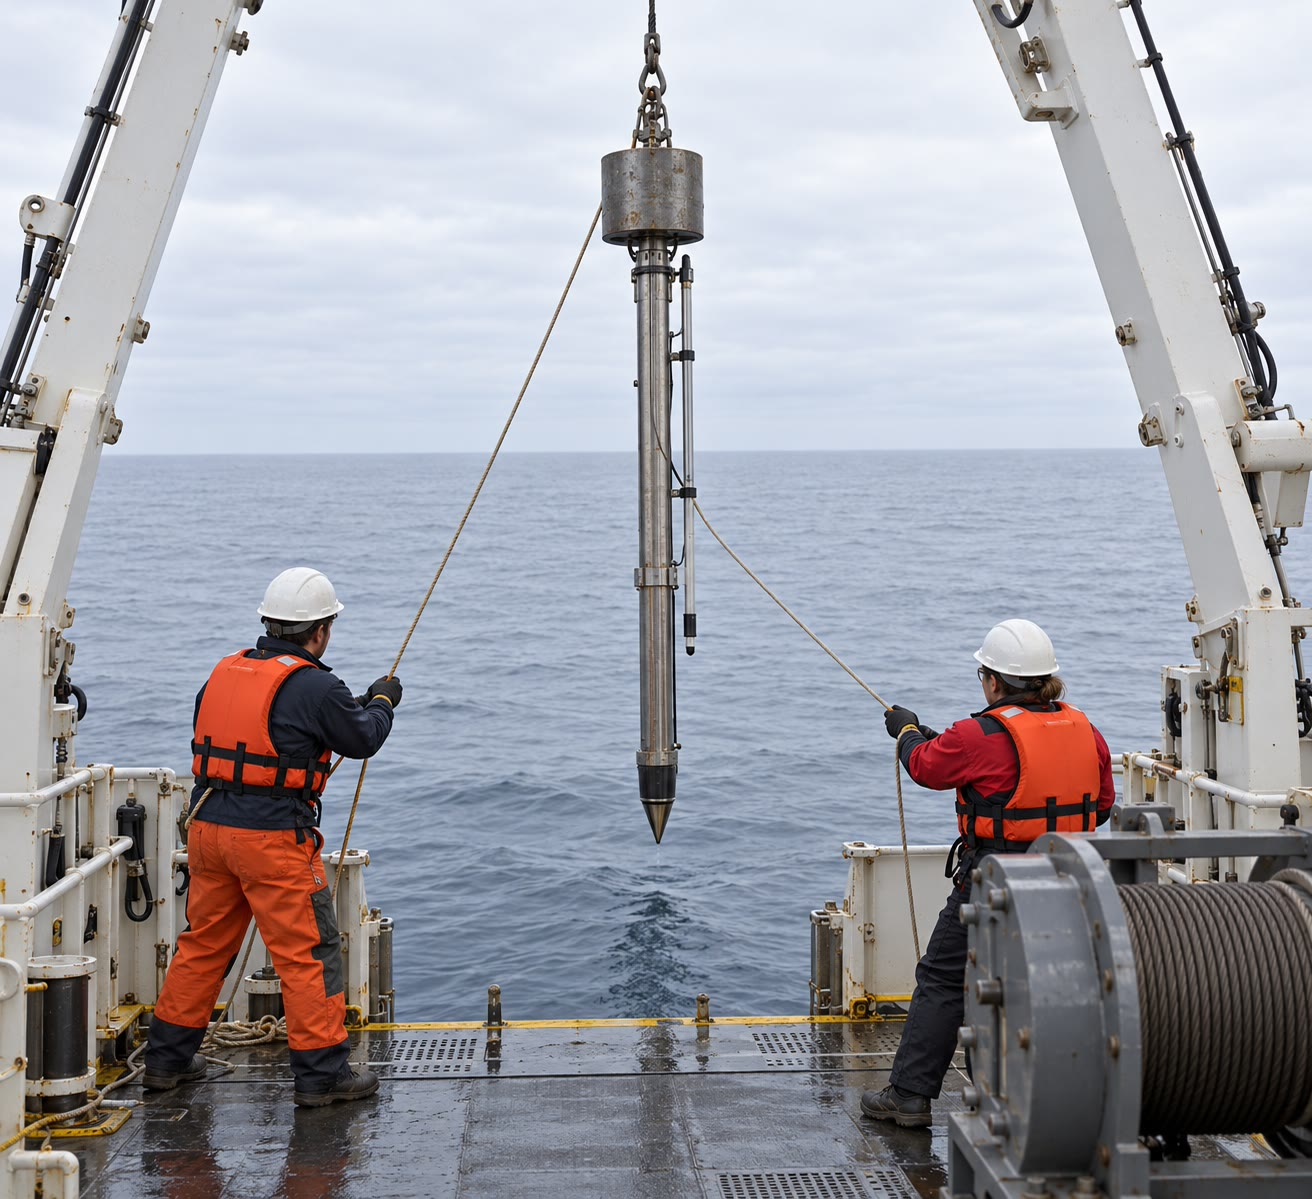
\includegraphics[width=\linewidth]{images/book5/ai/b3-heatflow-probe.jpg}

{\scriptsize Tombak aliran panas yang akan diturunkan dari buritan kapal
riset (ilustrasi buatan AI).}
\end{minipage}
\end{inthefield}

\section{Latihan}

\begin{exercise}[$\star$]\label{exo:b3:lithosphere-thermal-models:1}
Dengan $\kappa = \qty{e-6}{m^2.s^{-1}}$, hitung waktu konduktif $L^2/\kappa$
untuk $L = 1$, 10, dan \qty{100}{km}, dalam juta tahun.
\end{exercise}

\begin{exercise}[$\star$]\label{exo:b3:lithosphere-thermal-models:2}
Sebuah pegunungan terkikis dengan laju \qty{1}{mm/yr}, dan batuan naik melalui
\qty{30}{km} kerak bagian atas untuk menggantikannya. Dengan $\kappa = \qty{e-6}{m^2.s^{-1}}$,
hitung bilangan Péclet. Dapatkah geoterm pegunungan itu dihitung
dengan konduksi saja?
\end{exercise}

\begin{exercise}[$\star$]\label{exo:b3:lithosphere-thermal-models:3}
Dalam model setengah-ruang ($T_0 = 0$, $T_m = \qty{1450}{\celsius}$, $\kappa =
\qty{0.8e-6}{m^2.s^{-1}}$), hitung suhu \qty{10}{km} di bawah dasar laut
berumur \qty{5}{Ma} (\qty{1}{Ma} $= \qty{3.156e13}{s}$; $\operatorname{erf}
0.445 = 0.471$).
\end{exercise}

\begin{exercise}[$\star$]\label{exo:b3:lithosphere-thermal-models:4}
Dengan $C_q = \qty{490}{mW.m^{-2}.Ma^{1/2}}$, hitung aliran panas melalui
dasar laut berumur 1, 25, dan \qty{100}{Ma}. Manakah dari ketiganya
yang paling mungkin diremehkan oleh probe?
\end{exercise}

\begin{exercise}[$\star\star$]\label{exo:b3:lithosphere-thermal-models:5}
Dalam model setengah-ruang, suhu mencapai \qty{90}{\percent} dari $T_m$
ketika $\operatorname{erf}\eta = 0.9$, $\eta = 1.163$. Dengan $\kappa =
\qty{0.8e-6}{m^2.s^{-1}}$), hitung kedalaman itu pada 10, 40, dan \qty{100}{Ma}.
\end{exercise}

\begin{exercise}[$\star\star$]\label{exo:b3:lithosphere-thermal-models:6}
Dengan nilai-nilai dalam teks, model setengah-ruang memberikan $C =
\qty{370.5}{m.Ma^{-1/2}}$. Jika semua nilai lain dijaga tetap, koefisien ekspansi termal
berapa yang memberikan hasil pencocokan \qty{350}{m.Ma^{-1/2}}? Parameter lain
apa yang bisa diubah sebagai gantinya?
\end{exercise}

\begin{exercise}[$\star\star$]\label{exo:b3:lithosphere-thermal-models:7}
Hitung aliran panas asimtotik $kT_m/L$ model lempeng untuk $L =
\qty{95}{km}$, $T_m = \qty{1450}{\celsius}$, dan untuk $L = \qty{125}{km}$,
$T_m = \qty{1350}{\celsius}$, dengan $k = \qty{3.1}{W.m^{-1}.K^{-1}}$ untuk keduanya.
Mana yang lebih dekat dengan aliran panas dasar samudra tua yang dihitung dari $C_q/\sqrt t$
pada \qty{150}{Ma} dengan $C_q = \qty{490}{mW.m^{-2}.Ma^{1/2}}$?
\end{exercise}

\begin{exercise}[$\star\star$]\label{exo:b3:lithosphere-thermal-models:8}
Sebuah provinsi memiliki $q_0 = \qty{60}{mW.m^{-2}}$, $h_r = \qty{10}{km}$, dan $A_0h_r =
0.4\,q_0$. Hitung $A_0$, $q_m$, dan suhu di Moho, \qty{35}{km}
dalam, dengan $k = \qty{2.5}{W.m^{-1}.K^{-1}}$.
\end{exercise}

\begin{exercise}[$\star\star$]\label{exo:b3:lithosphere-thermal-models:9}
Dua pluton granit dari satu provinsi memberikan $q_0 = \qty{66}{mW.m^{-2}}$ dengan $A_0
= \qty{3.0}{\micro W.m^{-3}}$, dan $q_0 = \qty{48}{mW.m^{-2}}$ dengan $A_0 =
\qty{1.2}{\micro W.m^{-3}}$. Dengan asumsi keduanya terletak pada garis
\cref{prop:b3:lithosphere-thermal-models:exponential}, hitung $h_r$ dan $q_m$.
\end{exercise}

\begin{exercise}[$\star\star\star$]\label{exo:b3:lithosphere-thermal-models:10}
(a) Tunjukkan bahwa panas yang hilang melalui dasar laut antara umur 0 dan $t$, per
satuan luas, adalah $Q(t) = 2k(T_m - T_0)\sqrt{t/(\pi\kappa)}$ dalam
model setengah-ruang. (b) Tunjukkan bahwa penurunan adalah $d - d_r = \alpha Q/\bigl(c(\rho_m -
\rho_w)\bigr)$, dengan $c = k/(\rho_m\kappa)$ adalah kalor jenis. (c) Periksa
secara numerik pada \qty{40}{Ma} dengan nilai-nilai dalam teks.
\end{exercise}

\begin{exercise}[$\star\star\star$]\label{exo:b3:lithosphere-thermal-models:11}
Dalam model lempeng dari teks ($\tau = \qty{36.2}{Ma}$, $\rho_m\alpha T_mL/
\bigl(2(\rho_m - \rho_w)\bigr) = \qty{3104}{m}$), kedalaman yang dihitung dengan
suku Fourier pertama saja melampaui deret penuh, terutama oleh suku $n = 3$.
Hitung besar suku itu pada 1, 10, dan \qty{20}{Ma}, serta umur
setelah itu suku pertama saja berada dalam \qty{10}{m} dari deret penuh.
\end{exercise}

\begin{exercise}[$\star\star\star$]\label{exo:b3:lithosphere-thermal-models:12}
(a) Tunjukkan bahwa, pada geoterm dari \cref{prop:b3:lithosphere-thermal-models:exponential},
$T(z) \approx q_mz/k + A_0h_r^2/k$ untuk $z \gg h_r$. (b) Turunkan kedalaman
isoterm \qty{1300}{\celsius} untuk $q_0 = \qty{40}{mW.m^{-2}}$, dengan nilai-nilai
dari latihan 8. (c) Seberapa besar $q_m$ harus turun agar kedalaman itu mencapai
\qty{250}{km}, kedalaman akar cepat kraton?
\end{exercise}

\section{Soal: Empat puluh juta tahun dari punggungan}

\begin{problem}[{Soal akhir pekan --- model setengah-ruang dan model lempeng, kedalaman
samudra rekaan, dan ketebalan lempengnya}]
\label{pb:b3:lithosphere-thermal-models:1}
% values: calc/ch05.py; plate_cooling.py; honda04:gdh1, ps77:depth-age, data:b5-depth-age
Ambil $T_0 = 0$, $T_m = \qty{1450}{\celsius}$, $\kappa =
\qty{0.8e-6}{m^2.s^{-1}}$, $k = \qty{3.1}{W.m^{-1}.K^{-1}}$, $\alpha =
\qty{3.1e-5}{K^{-1}}$, $\rho_m = \qty{3300}{kg.m^{-3}}$, $\rho_w =
\qty{1030}{kg.m^{-3}}$, sebuah punggungan dengan kedalaman \qty{2500}{m}, dan \qty{1}{Ma} $=
\qty{3.156e13}{s}$.

\medskip\noindent\textbf{Bagian I --- Model setengah-ruang.}
\begin{enumerate}
  \item Hitung $\sqrt{\kappa t}$ pada 10 dan \qty{40}{Ma}.
  \item Hitung suhu \qty{20}{km} di bawah dasar laut pada kedua umur
        ($\operatorname{erf}0.6294 = 0.6266$, $\operatorname{erf}0.3147 =
        0.3437$).
  \item Isoterm \qty{1000}{\celsius} berada di tempat $\operatorname{erf}\eta =
        0.6897$, $\eta = 0.7174$. Hitung kedalamannya pada kedua umur, dan umur
        saat isoterm itu mencapai \qty{60}{km}.
  \item Hitung aliran panas pada kedua umur, dan $C_q$.
  \item Sebuah punggungan menyebar dengan laju \qty{25}{mm/yr} di setiap sisi. Hitung bilangan Péclet
        lempeng sepanjang \qty{95}{km}. Mengapa setiap kolom boleh didinginkan
        sendiri?
  \item Hitung waktu konduktif melintasi \qty{95}{km}. Apa yang dikatakannya tentang
        model setengah-ruang dasar laut berumur \qty{150}{Ma}?
\end{enumerate}

\medskip\noindent\textbf{Bagian II --- Penurunan.}
\begin{enumerate}[resume]
  \item Ingat kembali keseimbangan isostatik yang mengubah defisit suhu sebuah
        kolom menjadi penurunan, dan mengapa integral boleh dihitung sampai tak hingga
        di dalam setengah-ruang.
  \item Hitung $C$ dari hukum kedalaman--umur, serta kedalamannya pada 10 dan
        \qty{40}{Ma}.
  \item Kedalaman median dasar samudra nyata antara 40 dan \qty{45}{Ma}
        adalah \qty{4475}{m}, belum dikoreksi. Bandingkan dengan model pada
        \qty{42.5}{Ma}, dan daftarkan apa yang termasuk dalam median tetapi
        tidak dimasukkan dalam model.
  \item Sebesar apa $C$ akan berubah jika $T_m$ bernilai \qty{1350}{\celsius}?
        Bandingkan dengan \qty{350}{m.Ma^{-1/2}} hasil pencocokan.
  \item Mengapa aliran panas terukur pada dasar samudra muda berada di bawah $C_q/\sqrt t$?
\end{enumerate}

\medskip\noindent\textbf{Bagian III --- Lempengnya.} Ambil $L = \qty{95}{km}$.
\begin{enumerate}[resume]
  \item Hitung $\tau$ dan amplitudo $\rho_m\alpha T_mL/\bigl(2(\rho_m -
        \rho_w)\bigr)$.
  \item Hitung kedalaman pada \qty{40}{Ma} dengan suku $n = 1$, 3 dan 5.
  \item Seberapa besar suku pertama saja berbeda dari itu, dan mengapa
        sedikit sekali?
  \item Hitung selisih antara setengah-ruang dan lempeng pada 40 dan
        \qty{50}{Ma}, dan taksirlah dengan interpolasi linier umur saat selisih
        itu mencapai \qty{100}{m}.
  \item Hitung aliran panas lempeng pada \qty{40}{Ma}, dengan suku
        $n = 1$ sampai 3, dan bandingkan dengan setengah-ruang.
  \item Berikan kedalaman dan aliran panas asimtotiknya.
\end{enumerate}

\medskip\noindent\textbf{Bagian IV --- Samudra rekaan.} Di samudra rekaan
yang punggungannya berkedalaman \qty{2500}{m}, dasar laut, setelah dikoreksi terhadap sedimen
dan dengan mengabaikan gunung laut serta punggung, berkedalaman \qty{5700}{m} pada \qty{120}{Ma} dan
\qty{4800}{m} pada \qty{40}{Ma}. Nilai $L$ lempeng tidak diketahui; nilai lainnya
sama seperti di atas.
\begin{enumerate}[resume]
  \item Dengan hanya mempertahankan suku pertama deret Fourier, tuliskan kedalaman pada
        \qty{120}{Ma} sebagai fungsi $L$, dengan $\tau$ itu sendiri bergantung pada
        $L$.
  \item Selesaikan untuk $L$ dengan iterasi, mulai dari $L = \qty{100}{km}$:
        hitung $\tau$, lalu $L$ yang mencocokkan \qty{5700}{m} dengan $\tau$
        tersebut, dan ulangi.
  \item Dengan $L$ yang diperoleh, hitung kedalaman pada \qty{40}{Ma} dan
        bandingkan dengan setengah-ruang serta dengan \qty{4800}{m} terukur.
  \item Hitung $\tau$ untuk $L$ tersebut dan kedalaman asimtotik samudra ini.
  \item Setelah umur berapa dasar laut berada dalam jarak \qty{100}{m} dari
        kedalaman asimtotiknya?
  \item Berikan tebal $L$ lempeng yang sesuai dengan dasar samudra tua
        rekaan ini.
\end{enumerate}
\end{problem}
